\documentclass{standalone}
\usepackage{tikz, xcolor}
\usetikzlibrary{shapes,arrows}

\begin{document}

\begin{tikzpicture}[thick, scale=2.0]
\tikzstyle{vertexr}=[rectangle, draw=blue, thick, minimum size=14pt, inner sep=2pt]
\tikzstyle{vertexc}=[circle, draw=blue, thick, inner sep=2pt]
\tikzstyle{drawstyle}=[thick, ->]

\node[vertexr] (G0x0) at (0,0) {int a};
\node[vertexr] (G1x0) at (1,0) {int aa};
\node[vertexr] (G2x0) at (2,0) {void Func fox};
\node[vertexr] (G2x1) at (2,-1) {int fpa};
\node[vertexr] (G3x1) at (3,-1) {int fpaa};
\draw[drawstyle] (G2x1) -- (G3x1);
\draw[drawstyle] (G2x0) -- (G2x1);
\node[vertexr] (G4x1) at (4,-1) {Compound};
\node[vertexc] (G4x2) at (4,-2) {.};
\draw[drawstyle] (G4x1) -- (G4x2);
\node[vertexr] (G5x2) at (5,-2) {Call output};
\node[vertexr] (G5x3) at (5,-3) {fpa};
\draw[drawstyle] (G5x2) -- (G5x3);
\node[vertexr] (G6x2) at (6,-2) {Call output};
\node[vertexr] (G6x3) at (6,-3) {$*$};
\node[vertexr] (G6x4) at (6,-4) {fpaa};
\draw[drawstyle] (G6x3) -- (G6x4);
\draw[drawstyle] (G6x2) -- (G6x3);
\node[vertexr] (G7x2) at (7,-2) {Call output};
\node[vertexr] (G7x3) at (7,-3) {fpaa};
\node[vertexr] (G7x4) at (7,-4) {0};
\draw[drawstyle] (G7x3) -- (G7x4);
\draw[drawstyle] (G7x2) -- (G7x3);
\node[vertexr] (G8x2) at (8,-2) {Call output};
\node[vertexr] (G8x3) at (8,-3) {fpaa};
\node[vertexr] (G8x4) at (8,-4) {10};
\draw[drawstyle] (G8x3) -- (G8x4);
\draw[drawstyle] (G8x2) -- (G8x3);
\node[vertexr] (G9x2) at (9,-2) {Call outnl};
\draw[drawstyle] (G8x2) -- (G9x2);
\draw[drawstyle] (G7x2) -- (G8x2);
\draw[drawstyle] (G6x2) -- (G7x2);
\draw[drawstyle] (G5x2) -- (G6x2);
\draw[drawstyle] (G4x1) -- (G5x2);
\draw[drawstyle] (G2x0) -- (G4x1);
\node[vertexr] (G10x0) at (10,0) {void Func bat};
\node[vertexr] (G10x1) at (10,-1) {int fpa};
\node[vertexr] (G11x1) at (11,-1) {int fpaa};
\draw[drawstyle] (G10x1) -- (G11x1);
\draw[drawstyle] (G10x0) -- (G10x1);
\node[vertexr] (G12x1) at (12,-1) {Compound};
\node[vertexc] (G12x2) at (12,-2) {.};
\draw[drawstyle] (G12x1) -- (G12x2);
\node[vertexr] (G13x2) at (13,-2) {Call outputc};
\node[vertexr] (G13x3) at (13,-3) {'B'};
\draw[drawstyle] (G13x2) -- (G13x3);
\node[vertexr] (G14x2) at (14,-2) {Call fox};
\node[vertexr] (G14x3) at (14,-3) {fpa};
\node[vertexr] (G15x3) at (15,-3) {fpaa};
\draw[drawstyle] (G14x3) -- (G15x3);
\draw[drawstyle] (G14x2) -- (G14x3);
\draw[drawstyle] (G13x2) -- (G14x2);
\draw[drawstyle] (G12x1) -- (G13x2);
\draw[drawstyle] (G10x0) -- (G12x1);
\node[vertexr] (G16x0) at (16,0) {int Func th};
\node[vertexr] (G16x1) at (16,-1) {int fpa};
\draw[drawstyle] (G16x0) -- (G16x1);
\node[vertexr] (G17x1) at (17,-1) {Return};
\node[vertexr] (G17x2) at (17,-2) {fpa};
\draw[drawstyle] (G17x1) -- (G17x2);
\draw[drawstyle] (G16x0) -- (G17x1);
\node[vertexr] (G18x0) at (18,0) {int Func tha};
\node[vertexr] (G18x1) at (18,-1) {int fpaa};
\draw[drawstyle] (G18x0) -- (G18x1);
\node[vertexr] (G19x1) at (19,-1) {Return};
\node[vertexr] (G19x2) at (19,-2) {fpaa};
\node[vertexr] (G19x3) at (19,-3) {0};
\draw[drawstyle] (G19x2) -- (G19x3);
\draw[drawstyle] (G19x1) -- (G19x2);
\draw[drawstyle] (G18x0) -- (G19x1);
\node[vertexr] (G20x0) at (20,0) {void Func main};
\node[vertexr] (G20x1) at (20,-1) {int pa};
\node[vertexr] (G21x1) at (21,-1) {int paa};
\draw[drawstyle] (G20x1) -- (G21x1);
\draw[drawstyle] (G20x0) -- (G20x1);
\node[vertexr] (G22x1) at (22,-1) {Compound};
\node[vertexr] (G22x2) at (22,-2) {int b};
\node[vertexr] (G23x2) at (23,-2) {int bb};
\draw[drawstyle] (G22x2) -- (G23x2);
\draw[drawstyle] (G22x1) -- (G22x2);
\node[vertexr] (G24x2) at (24,-2) {=};
\node[vertexr] (G24x3) at (24,-3) {a};
\draw[drawstyle] (G24x2) -- (G24x3);
\node[vertexr] (G25x3) at (25,-3) {111};
\draw[drawstyle] (G24x2) -- (G25x3);
\node[vertexr] (G26x2) at (26,-2) {=};
\node[vertexr] (G26x3) at (26,-3) {aa};
\node[vertexr] (G26x4) at (26,-4) {0};
\draw[drawstyle] (G26x3) -- (G26x4);
\draw[drawstyle] (G26x2) -- (G26x3);
\node[vertexr] (G27x3) at (27,-3) {110};
\draw[drawstyle] (G26x2) -- (G27x3);
\node[vertexr] (G28x2) at (28,-2) {=};
\node[vertexr] (G28x3) at (28,-3) {aa};
\node[vertexr] (G28x4) at (28,-4) {10};
\draw[drawstyle] (G28x3) -- (G28x4);
\draw[drawstyle] (G28x2) -- (G28x3);
\node[vertexr] (G29x3) at (29,-3) {112};
\draw[drawstyle] (G28x2) -- (G29x3);
\node[vertexr] (G30x2) at (30,-2) {=};
\node[vertexr] (G30x3) at (30,-3) {b};
\draw[drawstyle] (G30x2) -- (G30x3);
\node[vertexr] (G31x3) at (31,-3) {222};
\draw[drawstyle] (G30x2) -- (G31x3);
\node[vertexr] (G32x2) at (32,-2) {=};
\node[vertexr] (G32x3) at (32,-3) {bb};
\node[vertexr] (G32x4) at (32,-4) {0};
\draw[drawstyle] (G32x3) -- (G32x4);
\draw[drawstyle] (G32x2) -- (G32x3);
\node[vertexr] (G33x3) at (33,-3) {220};
\draw[drawstyle] (G32x2) -- (G33x3);
\node[vertexr] (G34x2) at (34,-2) {=};
\node[vertexr] (G34x3) at (34,-3) {bb};
\node[vertexr] (G34x4) at (34,-4) {10};
\draw[drawstyle] (G34x3) -- (G34x4);
\draw[drawstyle] (G34x2) -- (G34x3);
\node[vertexr] (G35x3) at (35,-3) {222};
\draw[drawstyle] (G34x2) -- (G35x3);
\node[vertexr] (G36x2) at (36,-2) {Call fox};
\node[vertexr] (G36x3) at (36,-3) {a};
\node[vertexr] (G37x3) at (37,-3) {aa};
\draw[drawstyle] (G36x3) -- (G37x3);
\draw[drawstyle] (G36x2) -- (G36x3);
\node[vertexr] (G38x2) at (38,-2) {Call fox};
\node[vertexr] (G38x3) at (38,-3) {b};
\node[vertexr] (G39x3) at (39,-3) {bb};
\draw[drawstyle] (G38x3) -- (G39x3);
\draw[drawstyle] (G38x2) -- (G38x3);
\node[vertexr] (G40x2) at (40,-2) {Compound};
\node[vertexr] (G40x3) at (40,-3) {int c};
\node[vertexr] (G41x3) at (41,-3) {int cc};
\draw[drawstyle] (G40x3) -- (G41x3);
\draw[drawstyle] (G40x2) -- (G40x3);
\node[vertexr] (G42x3) at (42,-3) {=};
\node[vertexr] (G42x4) at (42,-4) {c};
\draw[drawstyle] (G42x3) -- (G42x4);
\node[vertexr] (G43x4) at (43,-4) {333};
\draw[drawstyle] (G42x3) -- (G43x4);
\node[vertexr] (G44x3) at (44,-3) {=};
\node[vertexr] (G44x4) at (44,-4) {cc};
\node[vertexr] (G44x5) at (44,-5) {0};
\draw[drawstyle] (G44x4) -- (G44x5);
\draw[drawstyle] (G44x3) -- (G44x4);
\node[vertexr] (G45x4) at (45,-4) {330};
\draw[drawstyle] (G44x3) -- (G45x4);
\node[vertexr] (G46x3) at (46,-3) {=};
\node[vertexr] (G46x4) at (46,-4) {cc};
\node[vertexr] (G46x5) at (46,-5) {10};
\draw[drawstyle] (G46x4) -- (G46x5);
\draw[drawstyle] (G46x3) -- (G46x4);
\node[vertexr] (G47x4) at (47,-4) {334};
\draw[drawstyle] (G46x3) -- (G47x4);
\node[vertexr] (G48x3) at (48,-3) {Call outnl};
\node[vertexr] (G49x3) at (49,-3) {Call fox};
\node[vertexr] (G49x4) at (49,-4) {a};
\node[vertexr] (G50x4) at (50,-4) {aa};
\draw[drawstyle] (G49x4) -- (G50x4);
\draw[drawstyle] (G49x3) -- (G49x4);
\node[vertexr] (G51x3) at (51,-3) {Call fox};
\node[vertexr] (G51x4) at (51,-4) {b};
\node[vertexr] (G52x4) at (52,-4) {bb};
\draw[drawstyle] (G51x4) -- (G52x4);
\draw[drawstyle] (G51x3) -- (G51x4);
\node[vertexr] (G53x3) at (53,-3) {Call fox};
\node[vertexr] (G53x4) at (53,-4) {c};
\node[vertexr] (G54x4) at (54,-4) {cc};
\draw[drawstyle] (G53x4) -- (G54x4);
\draw[drawstyle] (G53x3) -- (G53x4);
\draw[drawstyle] (G51x3) -- (G53x3);
\draw[drawstyle] (G49x3) -- (G51x3);
\draw[drawstyle] (G48x3) -- (G49x3);
\draw[drawstyle] (G46x3) -- (G48x3);
\draw[drawstyle] (G44x3) -- (G46x3);
\draw[drawstyle] (G42x3) -- (G44x3);
\draw[drawstyle] (G40x2) -- (G42x3);
\node[vertexr] (G55x2) at (55,-2) {Compound};
\node[vertexr] (G55x3) at (55,-3) {int d};
\node[vertexr] (G56x3) at (56,-3) {int dd};
\draw[drawstyle] (G55x3) -- (G56x3);
\draw[drawstyle] (G55x2) -- (G55x3);
\node[vertexr] (G57x3) at (57,-3) {=};
\node[vertexr] (G57x4) at (57,-4) {d};
\draw[drawstyle] (G57x3) -- (G57x4);
\node[vertexr] (G58x4) at (58,-4) {444};
\draw[drawstyle] (G57x3) -- (G58x4);
\node[vertexr] (G59x3) at (59,-3) {=};
\node[vertexr] (G59x4) at (59,-4) {dd};
\node[vertexr] (G59x5) at (59,-5) {0};
\draw[drawstyle] (G59x4) -- (G59x5);
\draw[drawstyle] (G59x3) -- (G59x4);
\node[vertexr] (G60x4) at (60,-4) {440};
\draw[drawstyle] (G59x3) -- (G60x4);
\node[vertexr] (G61x3) at (61,-3) {=};
\node[vertexr] (G61x4) at (61,-4) {dd};
\node[vertexr] (G61x5) at (61,-5) {10};
\draw[drawstyle] (G61x4) -- (G61x5);
\draw[drawstyle] (G61x3) -- (G61x4);
\node[vertexr] (G62x4) at (62,-4) {445};
\draw[drawstyle] (G61x3) -- (G62x4);
\node[vertexr] (G63x3) at (63,-3) {Call outnl};
\node[vertexr] (G64x3) at (64,-3) {Call fox};
\node[vertexr] (G64x4) at (64,-4) {a};
\node[vertexr] (G65x4) at (65,-4) {aa};
\draw[drawstyle] (G64x4) -- (G65x4);
\draw[drawstyle] (G64x3) -- (G64x4);
\node[vertexr] (G66x3) at (66,-3) {Call fox};
\node[vertexr] (G66x4) at (66,-4) {b};
\node[vertexr] (G67x4) at (67,-4) {bb};
\draw[drawstyle] (G66x4) -- (G67x4);
\draw[drawstyle] (G66x3) -- (G66x4);
\node[vertexr] (G68x3) at (68,-3) {Call fox};
\node[vertexr] (G68x4) at (68,-4) {d};
\node[vertexr] (G69x4) at (69,-4) {dd};
\draw[drawstyle] (G68x4) -- (G69x4);
\draw[drawstyle] (G68x3) -- (G68x4);
\node[vertexr] (G70x3) at (70,-3) {Call outnl};
\node[vertexr] (G71x3) at (71,-3) {Call bat};
\node[vertexr] (G71x4) at (71,-4) {a};
\node[vertexr] (G72x4) at (72,-4) {aa};
\draw[drawstyle] (G71x4) -- (G72x4);
\draw[drawstyle] (G71x3) -- (G71x4);
\node[vertexr] (G73x3) at (73,-3) {Call bat};
\node[vertexr] (G73x4) at (73,-4) {b};
\node[vertexr] (G74x4) at (74,-4) {bb};
\draw[drawstyle] (G73x4) -- (G74x4);
\draw[drawstyle] (G73x3) -- (G73x4);
\node[vertexr] (G75x3) at (75,-3) {Call bat};
\node[vertexr] (G75x4) at (75,-4) {d};
\node[vertexr] (G76x4) at (76,-4) {dd};
\draw[drawstyle] (G75x4) -- (G76x4);
\draw[drawstyle] (G75x3) -- (G75x4);
\draw[drawstyle] (G73x3) -- (G75x3);
\draw[drawstyle] (G71x3) -- (G73x3);
\draw[drawstyle] (G70x3) -- (G71x3);
\draw[drawstyle] (G68x3) -- (G70x3);
\draw[drawstyle] (G66x3) -- (G68x3);
\draw[drawstyle] (G64x3) -- (G66x3);
\draw[drawstyle] (G63x3) -- (G64x3);
\draw[drawstyle] (G61x3) -- (G63x3);
\draw[drawstyle] (G59x3) -- (G61x3);
\draw[drawstyle] (G57x3) -- (G59x3);
\draw[drawstyle] (G55x2) -- (G57x3);
\node[vertexr] (G77x2) at (77,-2) {Compound};
\node[vertexr] (G77x3) at (77,-3) {int e};
\node[vertexr] (G78x3) at (78,-3) {int ee};
\draw[drawstyle] (G77x3) -- (G78x3);
\draw[drawstyle] (G77x2) -- (G77x3);
\node[vertexr] (G79x3) at (79,-3) {=};
\node[vertexr] (G79x4) at (79,-4) {e};
\draw[drawstyle] (G79x3) -- (G79x4);
\node[vertexr] (G80x4) at (80,-4) {555};
\draw[drawstyle] (G79x3) -- (G80x4);
\node[vertexr] (G81x3) at (81,-3) {=};
\node[vertexr] (G81x4) at (81,-4) {ee};
\node[vertexr] (G81x5) at (81,-5) {0};
\draw[drawstyle] (G81x4) -- (G81x5);
\draw[drawstyle] (G81x3) -- (G81x4);
\node[vertexr] (G82x4) at (82,-4) {550};
\draw[drawstyle] (G81x3) -- (G82x4);
\node[vertexr] (G83x3) at (83,-3) {=};
\node[vertexr] (G83x4) at (83,-4) {ee};
\node[vertexr] (G83x5) at (83,-5) {10};
\draw[drawstyle] (G83x4) -- (G83x5);
\draw[drawstyle] (G83x3) -- (G83x4);
\node[vertexr] (G84x4) at (84,-4) {556};
\draw[drawstyle] (G83x3) -- (G84x4);
\node[vertexr] (G85x3) at (85,-3) {Call outnl};
\node[vertexr] (G86x3) at (86,-3) {Call fox};
\node[vertexr] (G86x4) at (86,-4) {a};
\node[vertexr] (G87x4) at (87,-4) {aa};
\draw[drawstyle] (G86x4) -- (G87x4);
\draw[drawstyle] (G86x3) -- (G86x4);
\node[vertexr] (G88x3) at (88,-3) {Call fox};
\node[vertexr] (G88x4) at (88,-4) {b};
\node[vertexr] (G89x4) at (89,-4) {bb};
\draw[drawstyle] (G88x4) -- (G89x4);
\draw[drawstyle] (G88x3) -- (G88x4);
\node[vertexr] (G90x3) at (90,-3) {Call fox};
\node[vertexr] (G90x4) at (90,-4) {e};
\node[vertexr] (G91x4) at (91,-4) {ee};
\draw[drawstyle] (G90x4) -- (G91x4);
\draw[drawstyle] (G90x3) -- (G90x4);
\node[vertexr] (G92x3) at (92,-3) {Call outnl};
\node[vertexr] (G93x3) at (93,-3) {Call bat};
\node[vertexr] (G93x4) at (93,-4) {a};
\node[vertexr] (G94x4) at (94,-4) {aa};
\draw[drawstyle] (G93x4) -- (G94x4);
\draw[drawstyle] (G93x3) -- (G93x4);
\node[vertexr] (G95x3) at (95,-3) {Call bat};
\node[vertexr] (G95x4) at (95,-4) {b};
\node[vertexr] (G96x4) at (96,-4) {bb};
\draw[drawstyle] (G95x4) -- (G96x4);
\draw[drawstyle] (G95x3) -- (G95x4);
\node[vertexr] (G97x3) at (97,-3) {Call bat};
\node[vertexr] (G97x4) at (97,-4) {e};
\node[vertexr] (G98x4) at (98,-4) {ee};
\draw[drawstyle] (G97x4) -- (G98x4);
\draw[drawstyle] (G97x3) -- (G97x4);
\draw[drawstyle] (G95x3) -- (G97x3);
\draw[drawstyle] (G93x3) -- (G95x3);
\draw[drawstyle] (G92x3) -- (G93x3);
\draw[drawstyle] (G90x3) -- (G92x3);
\draw[drawstyle] (G88x3) -- (G90x3);
\draw[drawstyle] (G86x3) -- (G88x3);
\draw[drawstyle] (G85x3) -- (G86x3);
\draw[drawstyle] (G83x3) -- (G85x3);
\draw[drawstyle] (G81x3) -- (G83x3);
\draw[drawstyle] (G79x3) -- (G81x3);
\draw[drawstyle] (G77x2) -- (G79x3);
\node[vertexr] (G99x2) at (99,-2) {Call outnl};
\node[vertexr] (G100x2) at (100,-2) {Call output};
\node[vertexr] (G100x3) at (100,-3) {Call th};
\node[vertexr] (G100x4) at (100,-4) {a};
\draw[drawstyle] (G100x3) -- (G100x4);
\draw[drawstyle] (G100x2) -- (G100x3);
\node[vertexr] (G101x2) at (101,-2) {Call output};
\node[vertexr] (G101x3) at (101,-3) {Call tha};
\node[vertexr] (G101x4) at (101,-4) {aa};
\draw[drawstyle] (G101x3) -- (G101x4);
\draw[drawstyle] (G101x2) -- (G101x3);
\node[vertexr] (G102x2) at (102,-2) {Call outnl};
\node[vertexr] (G103x2) at (103,-2) {Call bat};
\node[vertexr] (G103x3) at (103,-3) {Call th};
\node[vertexr] (G103x4) at (103,-4) {a};
\draw[drawstyle] (G103x3) -- (G103x4);
\node[vertexr] (G104x3) at (104,-3) {aa};
\draw[drawstyle] (G103x3) -- (G104x3);
\draw[drawstyle] (G103x2) -- (G103x3);
\node[vertexr] (G105x2) at (105,-2) {Call outnl};
\draw[drawstyle] (G103x2) -- (G105x2);
\draw[drawstyle] (G102x2) -- (G103x2);
\draw[drawstyle] (G101x2) -- (G102x2);
\draw[drawstyle] (G100x2) -- (G101x2);
\draw[drawstyle] (G99x2) -- (G100x2);
\draw[drawstyle] (G77x2) -- (G99x2);
\draw[drawstyle] (G55x2) -- (G77x2);
\draw[drawstyle] (G40x2) -- (G55x2);
\draw[drawstyle] (G38x2) -- (G40x2);
\draw[drawstyle] (G36x2) -- (G38x2);
\draw[drawstyle] (G34x2) -- (G36x2);
\draw[drawstyle] (G32x2) -- (G34x2);
\draw[drawstyle] (G30x2) -- (G32x2);
\draw[drawstyle] (G28x2) -- (G30x2);
\draw[drawstyle] (G26x2) -- (G28x2);
\draw[drawstyle] (G24x2) -- (G26x2);
\draw[drawstyle] (G22x1) -- (G24x2);
\draw[drawstyle] (G20x0) -- (G22x1);
\draw[drawstyle] (G18x0) -- (G20x0);
\draw[drawstyle] (G16x0) -- (G18x0);
\draw[drawstyle] (G10x0) -- (G16x0);
\draw[drawstyle] (G2x0) -- (G10x0);
\draw[drawstyle] (G1x0) -- (G2x0);
\draw[drawstyle] (G0x0) -- (G1x0);
\end{tikzpicture}
\end{document}
Number of warnings: 0
Number of errors: 0
